%%%%%%%%%%%%%%%%%%%%%%%%%%%%%%%%%%%%%%%%%
% Memo
% LaTeX Template
% Version 1.0 (30/12/13)
%
% This template has been downloaded from:
% http://www.LaTeXTemplates.com
%
% Original author:
% Rob Oakes (http://www.oak-tree.us) with modifications by:
% Vel (vel@latextemplates.com)
%
% License:
% CC BY-NC-SA 3.0 (http://creativecommons.org/licenses/by-nc-sa/3.0/)
%
%%%%%%%%%%%%%%%%%%%%%%%%%%%%%%%%%%%%%%%%%

\documentclass[letterpaper,11pt]{texMemo} % Set the paper size (letterpaper, a4paper, etc) and font size (10pt, 11pt or 12pt)

\usepackage{parskip} % Adds spacing between paragraphs
\usepackage[colorlinks]{hyperref}
\usepackage{graphicx}
\usepackage{float}
\usepackage{hyperref}
\usepackage{listings}
\hypersetup{citecolor=DeepPink4}
\hypersetup{linkcolor=red}
\hypersetup{urlcolor=blue}
\usepackage{cleveref}
\setlength{\parindent}{15pt} % Indent paragraphs

%----------------------------------------------------------------------------------------
%	MEMO INFORMATION
%----------------------------------------------------------------------------------------

\memoto{Dr.Randy Hoover} % Recipient(s)

\memofrom{Benjamin LeBrun, Benjamin Garcia} % Sender(s)

\memosubject{Lab Assignment 7: TC2 and Servo Control } % Memo subject

\memodate{\today} % Date, set to \today for automatically printing todays date

% \logo{\includegraphics[width=0.1\textwidth]{logo.png}} % Institution logo at the top right of the memo, comment out this line for no logo

%----------------------------------------------------------------------------------------

\begin{document}

\maketitle % Print the memo header information

%----------------------------------------------------------------------------------------
%	MEMO CONTENT
%----------------------------------------------------------------------------------------

\section*{Introduction}
For this lab, we utilized second internal timer to the Atmega328p to produce a PWM signal
to drive our robot car's servo. This required activating Timer 2 on control pin 3 and 
correctly setting it to output a 50 Hz control signal. This will be used to move the 
ultrasonic sensor 90 degrees left and right of our robot to effectively maneuvere around 
obsticles and walls.

\section*{Equipment}
The primary devices we used were:

\begin{itemize}
    \item Acrylic vehicle body with screws, assembled
    \item Elegoo Uno (chip: Atmega328p)
    \item HC-SR04 ultrasonic distance sensor
    \item SG 90 hobby servo motor
    \item 2 ICR18650 batteries with battery box
    \item Ribbon cables
    \item Host laptop with AVR-gcc 8-bit toolchain
    \item USB 2.0 A to B cable
\end{itemize}

\subsection*{Configuration}
Our robot vehicle was assembled according to Elegoo's instructions which can be found
on Elegoo's website at \url{https://www.elegoo.com/download/}. For this lab, we are
using the V3.0 version of the robot kit.

While the timers and configuration are similar to the configuration and driving of the 
DC motors using PWM modes from the Arduino's built in timers, for our servo we require a 
different operating frequency than our DC motor needs. In our case, we needed to generate 
a 50 Hz PWM signal from the second Timer, which required using Phase corrected mode instead 
of the DC motor's fast PWM mode and then writing a correct pulse width to the count registers.

This allows us to call a single function with the degree angle between 0 and 180 degrees with 0
being the leftmost position.

\begin{figure}[!ht]
\begin{center}
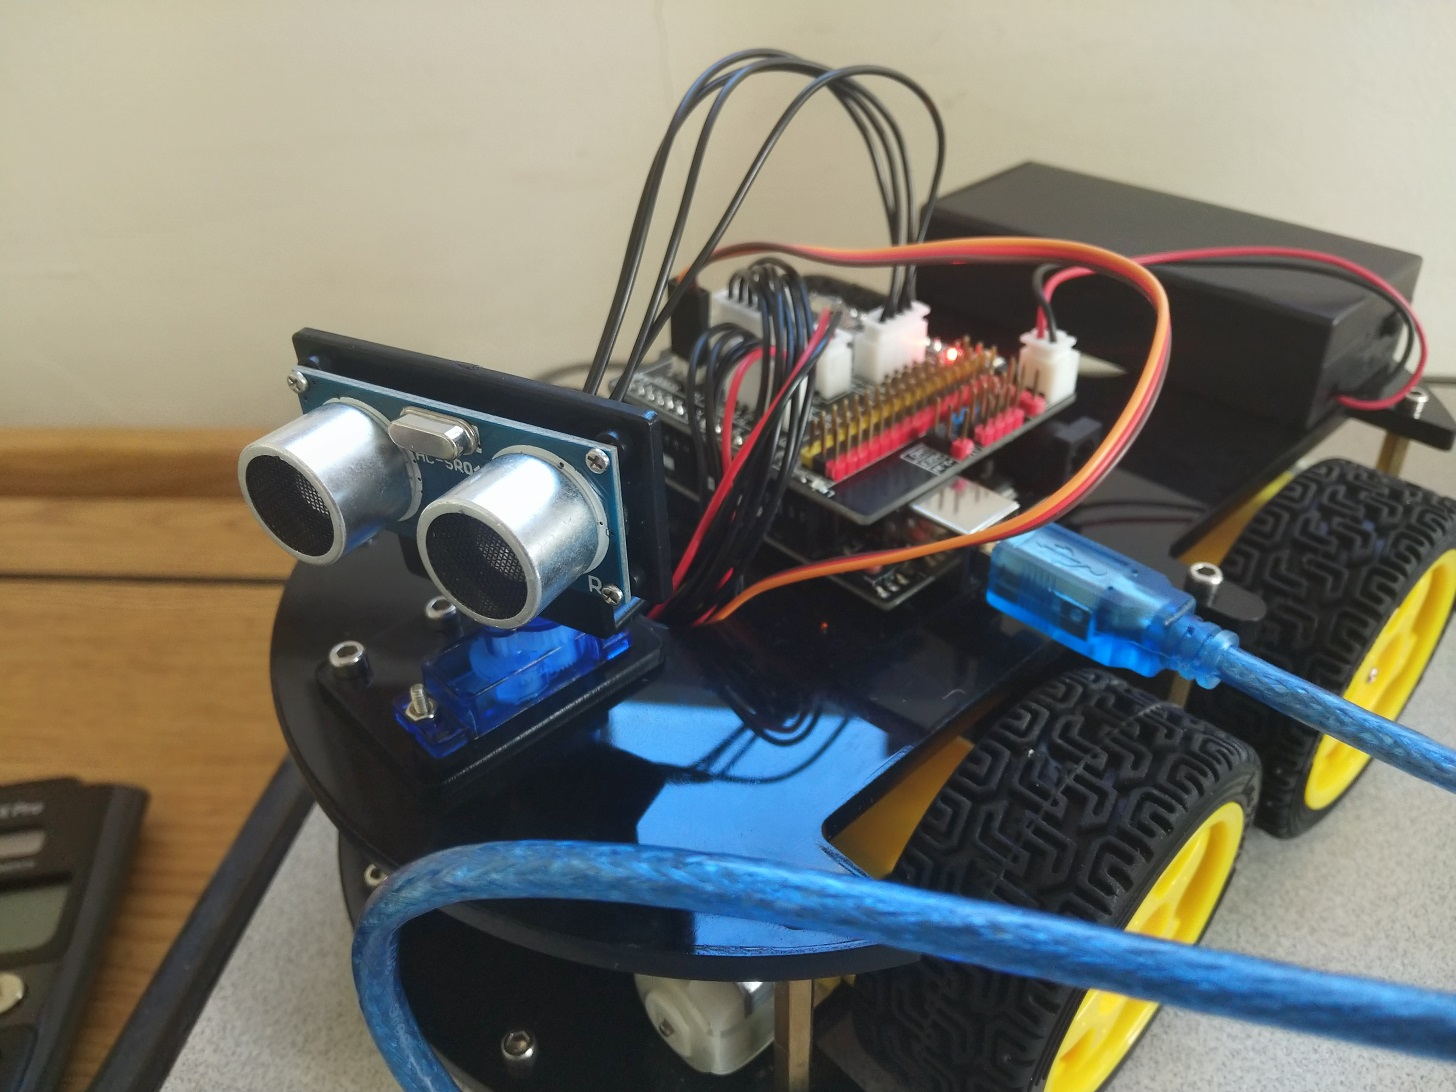
\includegraphics[width=\linewidth]{robot.jpg}
\end{center}
\caption{Servo with ultrasonic sensor assembly.}
\label{fig:f4}
\end{figure}

\section*{Implementation}
For this lab we are writing our own servo controller that should simply 
convert and assign the correct pwm mode for an approximate direction.

\subsection*{initServo}
Initializes timer 2 and sets the phase to the correct 50 Hz signal. 
Also sets any pins needed by the servo.

\subsection*{moveServo}
Takes in a degree angle, maps to a PWM value then assigns to the PWM 
pin controlling the servo.

\subsection*{mapAngle}
Takes in an angle and returns a mapped PWM value for the angle, exposed 
to allow us to read and debug.

\section*{Discussion}


\section*{Responses}
\begin{enumerate}
\item Not all hobby servos are made equal. Yours may have different lower/upper bounds than
1ms or 2ms. What is your servo’s pulse-width response range? How many discrete steps
does this translate to in your code?



\item  The Arduino libraries allow for any PWM pin to drive servos precisely, not just timer/-
counter 1. How does the Arduino source code manage this feat? You will have to do some
digging and exposition here.

In the internal analogWrite() function inside the arduino libraries, the analog function only works 
on pins connected to a timer. Otherwise the arduino will switch to a digital in/out write.

Otherwise, for each induvidual pin, the internal code attempts to read the correct pin/timer combo 
with a switch statement and will then configure quickly the correct PWM mode that takes in a 
value between 0 and 255 that can be directly written to the corresponding OCRXN register. To save time 
and create simplicity, in processing this correct pin/timer combo, if the values are 0 or 255, 
the analogWrite function defaults to just writing to those pins digitally high or low.


\end{enumerate} 

\newpage
\section*{Appendices}
Table of contents:
\begin{itemize}
    \item main.c - entry, initialization and drive instructions
    \item bit\_macros.h - bit manipulations macros
    \item globals.h - global variables needed by libraries using timers
    \item pcint.h - Pin change interrupt header for ultrasonic sensor
    \item pcint.c - Pin change interrupt code for ultrasonic sensor
    \item pin\_map.h - Pin map header for device
    \item robotio.h - UART control header
    \item robotio.c - UART control code
    \item servo.h - Servo control library
    \item servo.c - Servo control code
    \item timers.h - Timers control library
    \item timers.c - Timers control code
    \item ultrasonic.h - Ultrasonic header file
    \item ultrasonic.c - Ultrasonic code file
\end{itemize}
\newpage

\section*{Appendix A: main.c}
\begin{tiny}
\lstinputlisting{../main.c}
\end{tiny}
\newpage

\section*{Appendix B: bit\_macros.h}
\begin{tiny}
\lstinputlisting{../bit_macros.h}
\end{tiny}
\newpage

\section*{Appendix C: globals.h}
\begin{tiny}
\lstinputlisting{../globals.h}
\end{tiny}
\newpage

\section*{Appendix F: pcint.h}
\begin{tiny}
\lstinputlisting{../pcint.c}
\end{tiny}
\newpage

\section*{Appendix G: pcint.c}
\begin{tiny}
\lstinputlisting{../pcint.c}
\end{tiny}
\newpage

\section*{Appendix G: pin\_map.h}
\begin{tiny}
\lstinputlisting{../pin_map.h}
\end{tiny}
\newpage

\section*{Appendix H: robotio.h}
\begin{tiny}
\lstinputlisting{../robotio.h}
\end{tiny}
\newpage

\section*{Appendix H: robotio.c}
\begin{tiny}
\lstinputlisting{../robotio.c}
\end{tiny}
\newpage

\section*{Appendix H: servo.h}
\begin{tiny}
\lstinputlisting{../servo.h}
\end{tiny}
\newpage

\section*{Appendix H: servo.c}
\begin{tiny}
\lstinputlisting{../servo.c}
\end{tiny}
\newpage

\section*{Appendix H: timers.h}
\begin{tiny}
\lstinputlisting{../timers.h}
\end{tiny}
\newpage

\section*{Appendix H: timers.c}
\begin{tiny}
\lstinputlisting{../timers.c}
\end{tiny}
\newpage

\section*{Appendix H: ultrasonic.h}
\begin{tiny}
\lstinputlisting{../ultrasonic.h}
\end{tiny}
\newpage

\section*{Appendix H: ultrasonic.c}
\begin{tiny}
\lstinputlisting{../ultrasonic.c}
\end{tiny}
\newpage

\end{document}
\grid
